\documentclass{article}
\usepackage{graphicx} % Required for inserting images
\usepackage[T1]{fontenc}
\usepackage[a4paper,top=2cm,bottom=2cm,left=3cm,right=3cm,marginparwidth=1.75cm]{geometry}
\usepackage[polish]{babel}
\usepackage[MeX]{polski}
\usepackage{indentfirst}
\usepackage{caption}
\usepackage{float}
\usepackage[export]{adjustbox}
\usepackage{graphicx}
\usepackage[utf8]{inputenc}
\usepackage{polski}
\usepackage{geometry}
\usepackage{array}
\usepackage[utf8]{inputenc}
\usepackage{longtable}
\usepackage{booktabs}
\usepackage{multirow}
\usepackage{tabularx}
\usepackage{xltabular}
\usepackage{subcaption}

\usepackage[a4paper,top=2cm,bottom=2cm,left=3cm,right=3cm,marginparwidth=1.75cm]{geometry}

% Useful packages
\usepackage{amsmath}
\usepackage{graphicx}
\usepackage[colorlinks=true, allcolors=black]{hyperref}

\title{
    \centerline{
\includegraphics[width = 16cm]{PW_MiNI_PL_czarny_RGB.png}}
    \vspace{0.7cm}
    \textbf{Generowanie fraktalnych krajobrazów}
}

\author{Mateusz Wiktorzak, Wojciech Łapan}
\date{styczeń 2025}

\begin{document}

\maketitle

\tableofcontents

\vspace{0.4cm}

\section{Wstęp}

Interpolacja fraktalna to metoda generowania powierzchni lub funkcji o cechach fraktalnych, która wykorzystuje właściwości samopodobieństwa do interpolowania wartości pomiędzy danymi punktami. Jest to szczególny rodzaj interpolacji, który zamiast tworzyć gładkie przejścia między punktami, generuje bardziej złożone, „szorstkie” struktury, przypominające naturalne krajobrazy, linie brzegowe czy powierzchnie terenu.

\subsection{Kluczowe cechy interpolacji fraktalnej}

\begin{itemize}
    \item \textbf{Samopodobieństwo}: Struktury generowane przez interpolację fraktalną wykazują podobieństwo w różnych skalach (zoomowanie ujawnia te same wzory, niezależnie od poziomu szczegółowości).
    \item \textbf{Losowość kontrolowana parametrami}: Zmienność (np. „szorstkość” powierzchni) jest kontrolowana przez parametry, takie jak współczynnik szorstkości (\textit{roughness}) lub wymiar fraktalny (\textit{fractal dimension}).
    \item \textbf{Dodawanie szczegółów}: Interpolacja fraktalna dodaje szczegóły na różnych poziomach, przy jednoczesnym zachowaniu podstawowego kształtu wynikającego z punktów początkowych.
\end{itemize}

\subsection{Jak działa interpolacja fraktalna?}


\begin{enumerate}
    \item \textbf{Punkty kontrolne}: Na początku mamy zestaw punktów kontrolnych (np. 2D na płaszczyźnie lub 3D na powierzchni), które definiują podstawowy kształt funkcji lub powierzchni.
    \item \textbf{Zachowanie interpolacji klasycznej}: Interpolacja fraktalna zachowuje własności klasycznej interpolacji — wszystkie punkty kontrolne są dokładnie odwzorowywane.
    \item \textbf{Dodanie perturbacji}: Pomiędzy punktami kontrolnymi wprowadza się perturbacje (zakłócenia), które są losowe, ale zgodne z samopodobieństwem fraktalnym.
    \item \textbf{Rekurencja}: Proces jest stosowany wielokrotnie w sposób rekurencyjny, przy czym każda iteracja dodaje coraz drobniejsze szczegóły do generowanej funkcji lub powierzchni.
\end{enumerate}

\vspace{0.5cm}

\subsection{Wymiary Minkowskiego i Hausdorffa - Generowanie Krajobrazów Fraktalnych}

Fraktalne krajobrazy generowane metodą Diamond-Square charakteryzują się nieregularnością i złożonością, które można opisać za pomocą wymiarów Minkowskiego i Hausdorffa. Te miary pozwalają na matematyczną analizę właściwości fraktalnych wygenerowanych struktur.

\subsubsection*{Wymiar Minkowskiego}

Wymiar Minkowskiego, znany również jako wymiar pudełkowy, opisuje sposób, w jaki liczba pudełek \(N(\epsilon)\), potrzebnych do pokrycia krajobrazu, zmienia się wraz z rozmiarem \(\epsilon\). W przypadku generowanego krajobrazu algorytm Diamond-Square pozwala na analizę jego "szorstkości" poprzez badanie tej zależności.

\[
D_M = \lim_{\epsilon \to 0} \frac{\log N(\epsilon)}{\log(1/\epsilon)}
\]

Przybliżony wymiar Minkowskiego można obliczyć, stosując pokrycie siatki różnymi rozmiarami pudełek i zliczając, ile z nich zawiera wartości różne od zera.

\subsubsection*{Wymiar Hausdorffa}

Wymiar Hausdorffa jest bardziej precyzyjną miarą nieregularności i złożoności. Opisuje, jak powierzchnia fraktalna skaluje się w przestrzeni i może być oszacowany jako nachylenie prostej w analizie log-log zależności \(N(\epsilon)\) od \(\epsilon\):

\[
D_H = \inf \{d \geq 0 : \sum_i \epsilon_i^d < \infty\}
\]

W praktyce, wymiar Hausdorffa jest często zbliżony do wymiaru Minkowskiego dla generowanych krajobrazów, ale jest obliczany na podstawie bardziej precyzyjnej analizy skalowania. W przypadku fraktalnych krajobrazów generowanych metodą Diamond-Square można oszacować ten wymiar jako nachylenie liniowej regresji logarytmicznej.

\subsubsection*{Zastosowanie do Krajobrazów Fraktalnych}

Analiza wymiarów Minkowskiego i Hausdorffa dostarcza narzędzi do badania matematycznych właściwości generowanych krajobrazów oraz oceny wpływu parametrów algorytmu na uzyskiwane struktury.

\newpage
\section{Implementacja interpolacji fraktalnej - alogrytm Diamon-Square}

Algorytm Diamond-Square jest techniką generowania powierzchni fraktalnych, często używaną do tworzenia realistycznych map wysokości terenu w grach komputerowych i symulacjach.

\subsection{Opis algorytmu}

Algorytm Diamond-Square składa się z dwóch głównych kroków: kroku diamentowego (diamond step) i kroku kwadratowego (square step), które są wykonywane iteracyjnie w celu wygenerowania powierzchni o fraktalnych właściwościach. Składa się z następujących kroków:

\begin{enumerate}
    \item \textbf{Inicjalizacja:} Tworzony jest kwadratowy siatka o rozmiarze \( \text{size} \times \text{size} \), w której wartości wysokości są początkowo ustawione na 0. Następnie w czterech rogach siatki losowane są wartości z przedziału [-1, 1].
    \item \textbf{Krok diamentowy:} Dla każdej "diamentowej"\ komórki (wyznaczonej na podstawie czterech sąsiednich komórek) obliczana jest średnia ich wartości, do której dodawany jest losowy element z przedziału \([-scale, scale]\), aby wprowadzić losową zmienność.
    \item \textbf{Krok kwadratowy:} W każdej "kwadratowej"\ komórce, która jest średnią swoich czterech sąsiadów, również wprowadzana jest losowa zmienność, oparta na średniej wysokości sąsiednich komórek.
    \item \textbf{Zmniejszanie kroku:} Rozmiar kroku (\texttt{step\_size}) jest stopniowo zmniejszany, a zmienność (\texttt{scale}) jest redukowana, aby osiągnąć bardziej szczegółowe i gładkie wyniki.
\end{enumerate}

\begin{figure}[H]
    \centering
    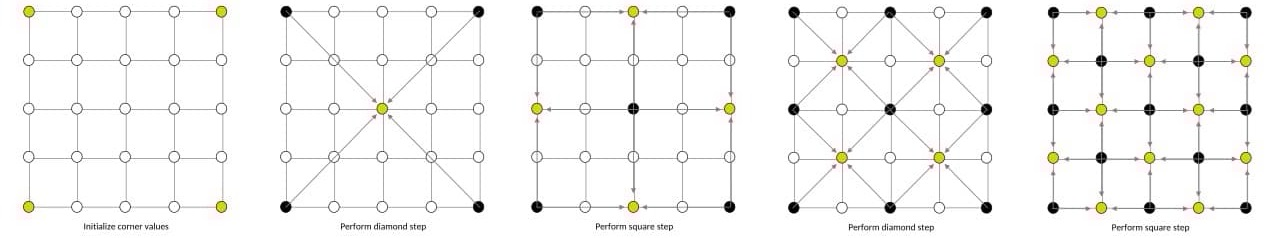
\includegraphics[width=1\linewidth]{rekurencja.jpg}
    \label{rekurencja}
\end{figure}

\subsection{Kod w pythonie}

\begin{verbatim}
import numpy as np
import matplotlib.pyplot as plt

def diamond_square(size, roughness):
    """
    Generates a 2D heightmap using the Diamond-Square algorithm.

    Parameters:
        size (int): The size of the grid (must be 2^n + 1).
        roughness (float): The roughness factor controlling terrain variation.

    Returns:
        np.ndarray: A 2D numpy array representing the heightmap.
    """
    # Initialize the grid
    grid = np.zeros((size, size))

    # Seed the corners
    grid[0, 0] = np.random.uniform(-1, 1)
    grid[0, -1] = np.random.uniform(-1, 1)
    grid[-1, 0] = np.random.uniform(-1, 1)
    grid[-1, -1] = np.random.uniform(-1, 1)

    step_size = size - 1
    scale = roughness

    while step_size > 1:
        half_step = step_size // 2

        # Diamond step
        for x in range(0, size - 1, step_size):
            for y in range(0, size - 1, step_size):
                avg = (grid[x, y] + grid[x + step_size, y] +
                       grid[x, y + step_size] + grid[x + step_size, y + step_size]) / 4.0
                grid[x + half_step, y + half_step] = avg + np.random.uniform(-scale, scale)

        # Square step
        for x in range(0, size, half_step):
            for y in range((x + half_step) % step_size, size, step_size):
                neighbors = []
                if x - half_step >= 0:
                    neighbors.append(grid[x - half_step, y])
                if x + half_step < size:
                    neighbors.append(grid[x + half_step, y])
                if y - half_step >= 0:
                    neighbors.append(grid[x, y - half_step])
                if y + half_step < size:
                    neighbors.append(grid[x, y + half_step])
                
                avg = sum(neighbors) / len(neighbors)
                grid[x, y] = avg + np.random.uniform(-scale, scale)

        # Reduce the scale for smaller steps
        step_size //= 2
        scale *= roughness

    return grid
\end{verbatim}

\subsection*{Parametry}

\begin{itemize}
    \item \textbf{size}: Rozmiar siatki, który musi być liczba postaci \(2^n + 1\), np. 33, 65, 129, itd.
    \item \textbf{roughness}: Współczynnik chropowatości, który kontroluje zakres zmienności terenu.
\end{itemize}

\subsection*{Generowanie i wizualizacja mapy}

Kod generuje mapę wysokości przy użyciu algorytmu Diamond-Square, a następnie wyświetla ją jako obrazek przy użyciu biblioteki \texttt{matplotlib}. Zastosowana mapa kolorów to \texttt{terrain}, która jest typowa dla reprezentacji terenów, ale można też użyć innych np. \textit{Blues}, czy \textit{YlOrBr}.

\begin{verbatim}
# Parameters
n = 10
size = 2**n + 1  # Must be 2^n + 1 (e.g., 33, 65, 129, ...)
roughness = 0.7
cmap = 'terrain' # examples: 'terrain', 'Blues', 'YlOrBr'

# Generate heightmap
heightmap = diamond_square(size, roughness)

# Visualize the heightmap
plt.figure(figsize=(10, 10))
plt.imshow(heightmap, cmap=cmap, origin='lower')
plt.colorbar(label='Height')
plt.title('Fractal Landscape - Diamond-Square Algorithm')
plt.show()
\end{verbatim}

\newpage

\subsection{Wyniki}

Poniżej prezentujemy kilka ciekawych wygenerowanych obrazków. Ich parametry oraz to co przedstawiają opisuje poniższa tabela. \\

\begin{longtable}{|p{0.05\linewidth}|p{0.1\linewidth}|p{0.1\linewidth}|p{0.1\linewidth}|p{0.5\linewidth}|}
    \hline
    \textbf{L.p.} & \textbf{size} & \textbf{roughness} & \textbf{cmap} & \textbf{interpretacja}\\
    \hline
    \endhead
    1. & 10 & 0.65 & terrain & ukształtowanie terenu \\
    \hline
    2. & 10 & 0.7 & Blues & niebo \\
    \hline
    3. & 10 & 0.9 & YlOrBr & słońce/wybuch \\
    \hline
\caption{Przykłady wygenerowanych fraktalnych krajobrazów}
\end{longtable}

\begin{figure}[H]
    \centering
    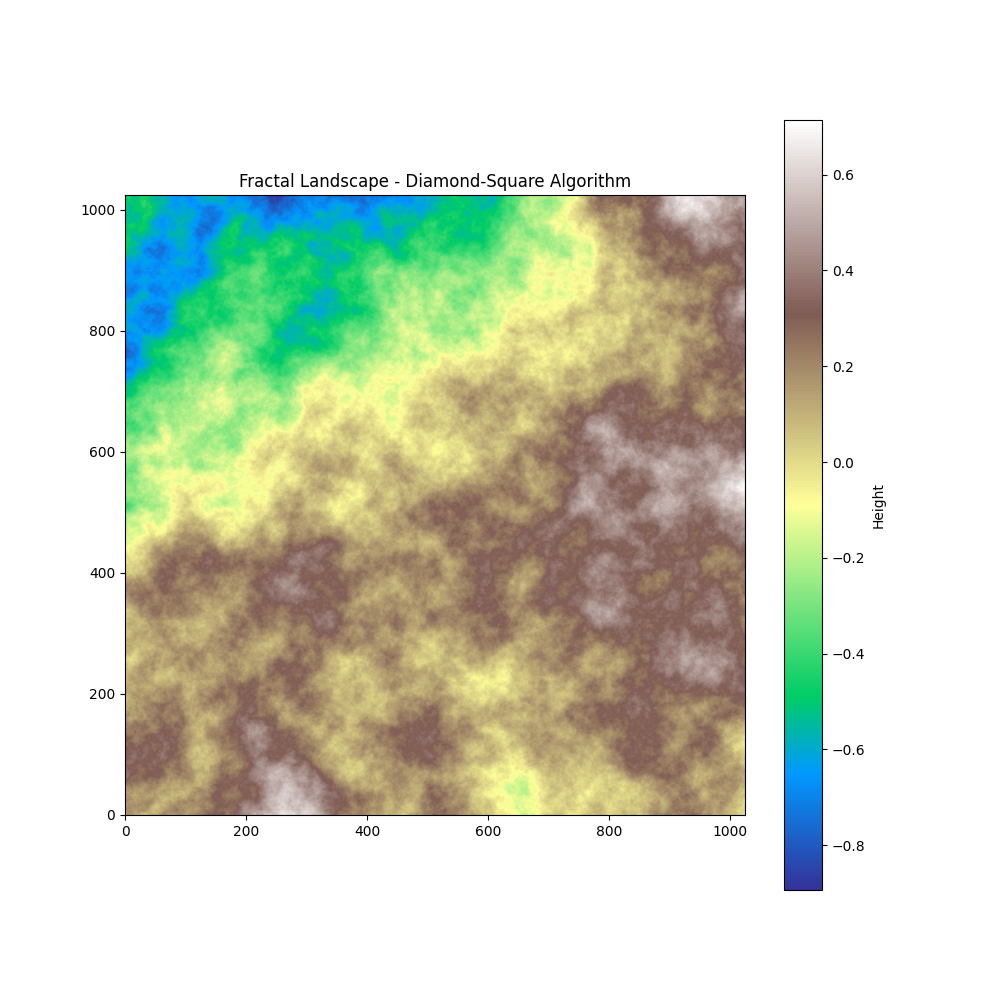
\includegraphics[width=0.7\linewidth]{terrain_10_0.65.png}
    \caption{Ukształtowanie terenu}
\end{figure}

\begin{figure}[H]
    \centering
    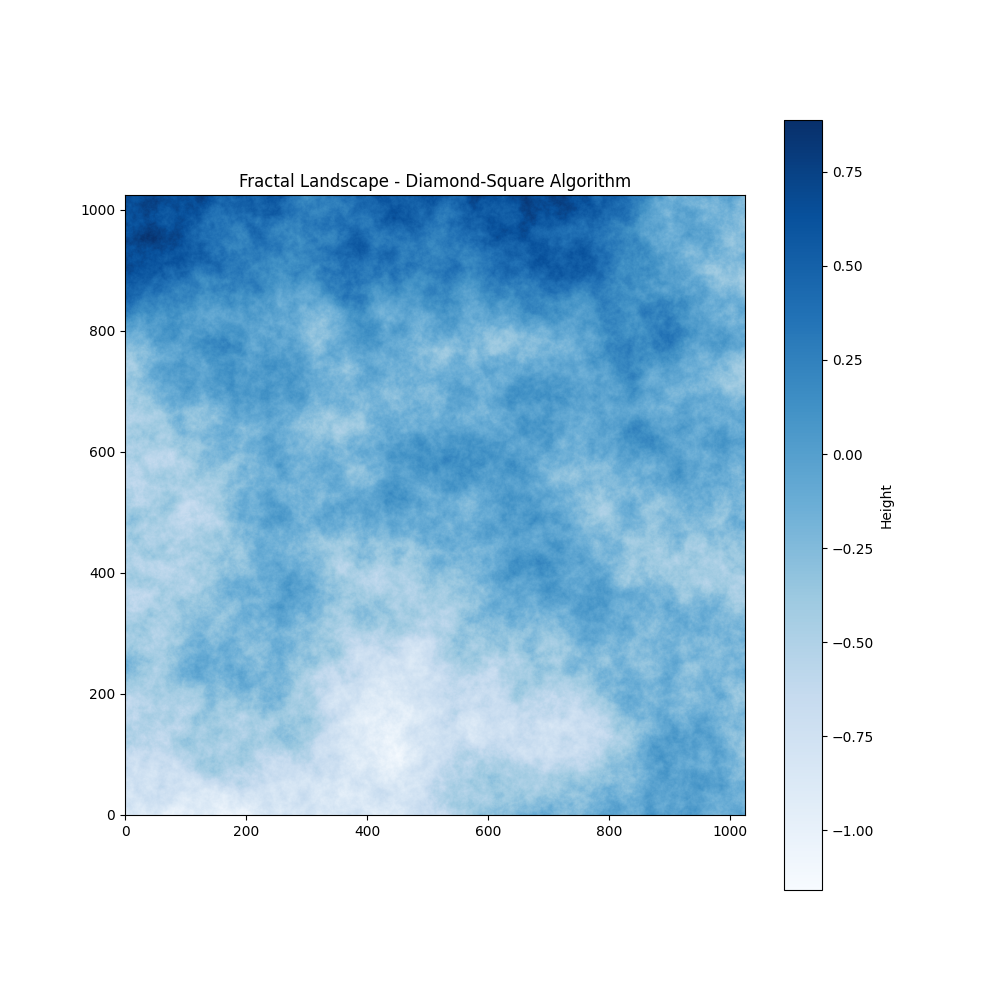
\includegraphics[width=0.7\linewidth]{Blues_10_0.7.png}
    \caption{Niebo}
\end{figure}

\begin{figure}[H]
    \centering
    \includegraphics[width=0.7\linewidth]{YlOrBr_10_0.9.png}
    \caption{Słońce/Wybuch}
\end{figure}
\newpage
\subsection*{Analiza wpływu parametrów}

Poniżej widoczny jest wpływ parametru \textit{size}. Wraz z jego wzrostem obraz ma większą rozdzielczość.

\begin{figure}[H]
    \centering
    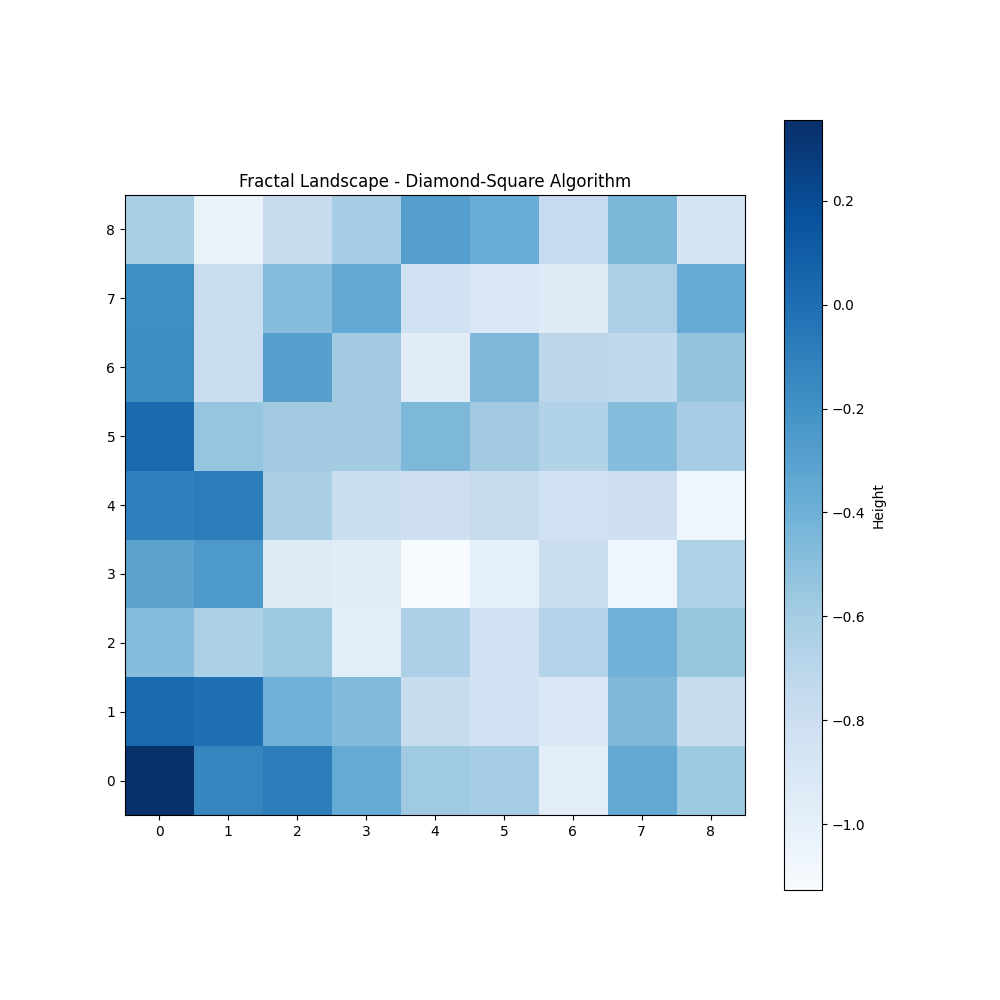
\includegraphics[width=0.7\linewidth]{Blues_3_0.7.png}
    \caption{Size = 3}
\end{figure}

\begin{figure}[H]
    \centering
    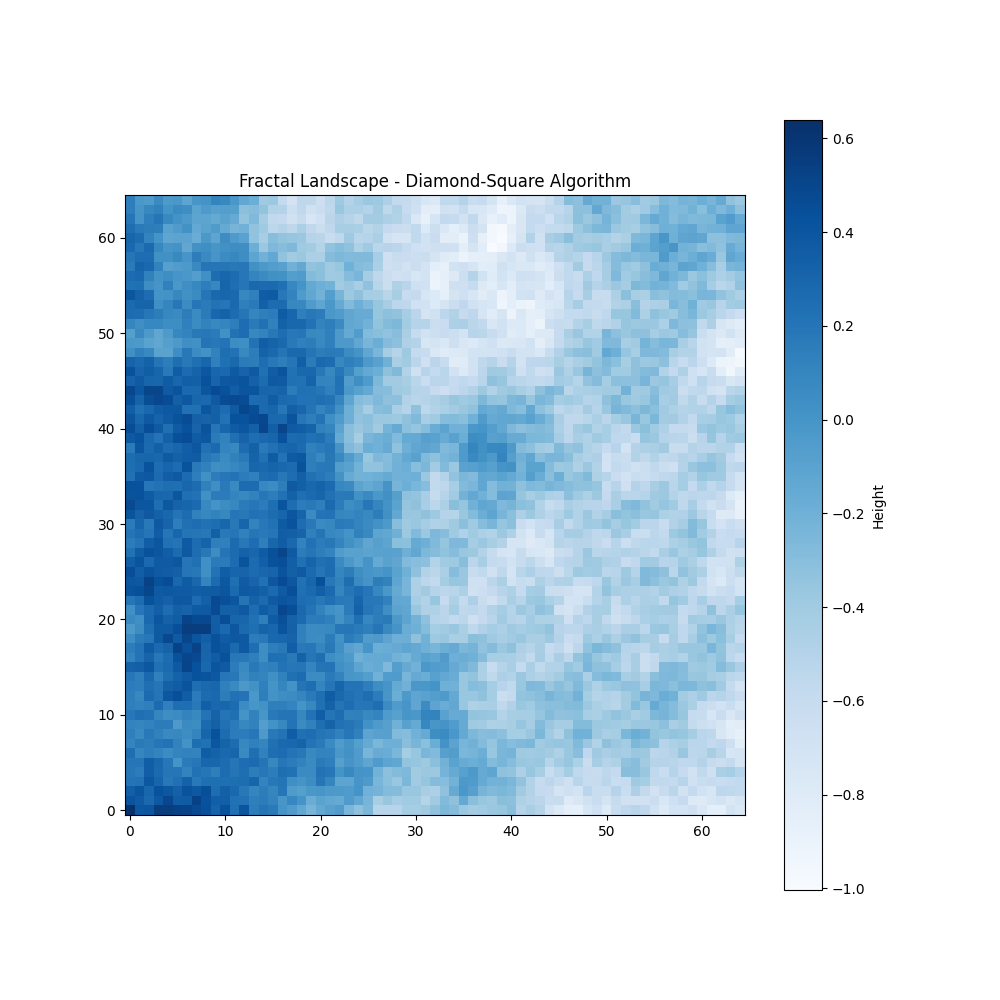
\includegraphics[width=0.7\linewidth]{Blues_6_0.7.png}
    \caption{Size = 6}
\end{figure}

\begin{figure}[H]
    \centering
    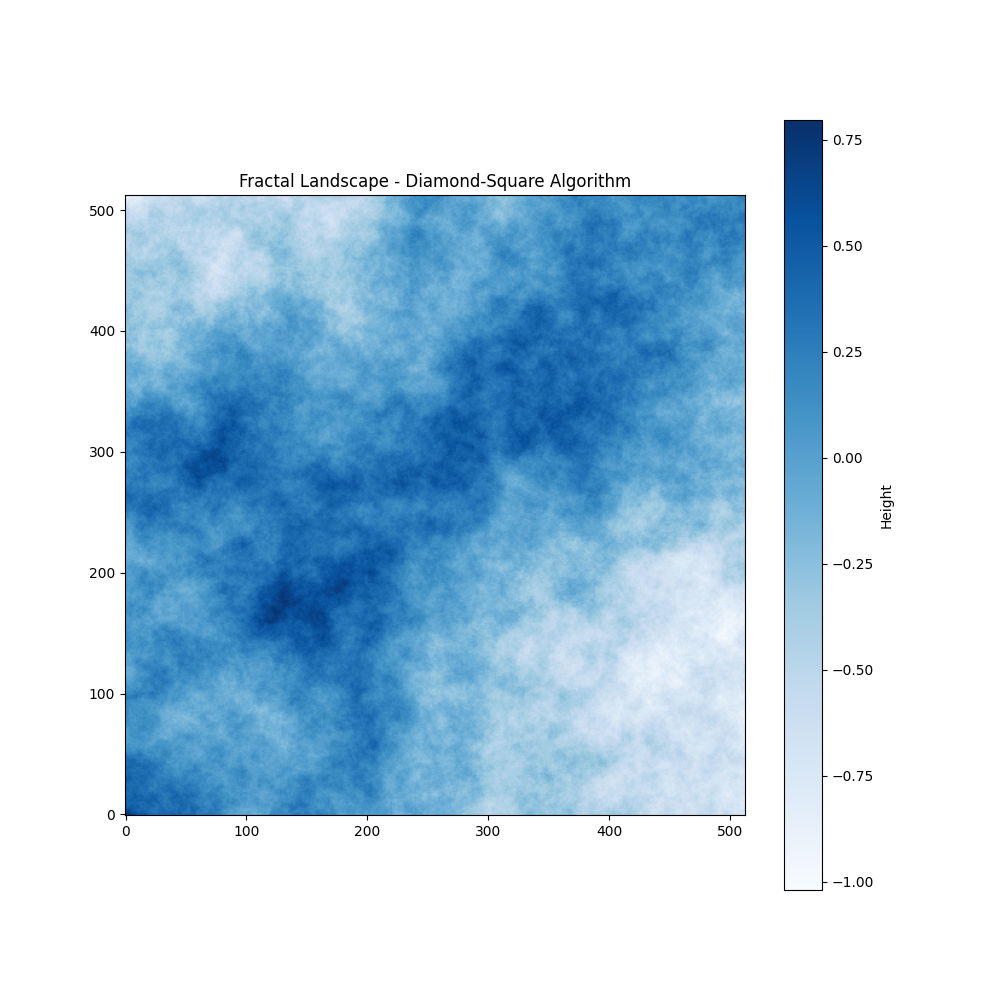
\includegraphics[width=0.7\linewidth]{Blues_9_0.7.png}
    \caption{Size = 9}
\end{figure}

\newpage

Następnym parametrem jest \textit{roughness (chropowatość)}. Wraz z jego wzrostem zwiększa się nieregularność grafiki. 

\begin{figure}[H]
    \centering
    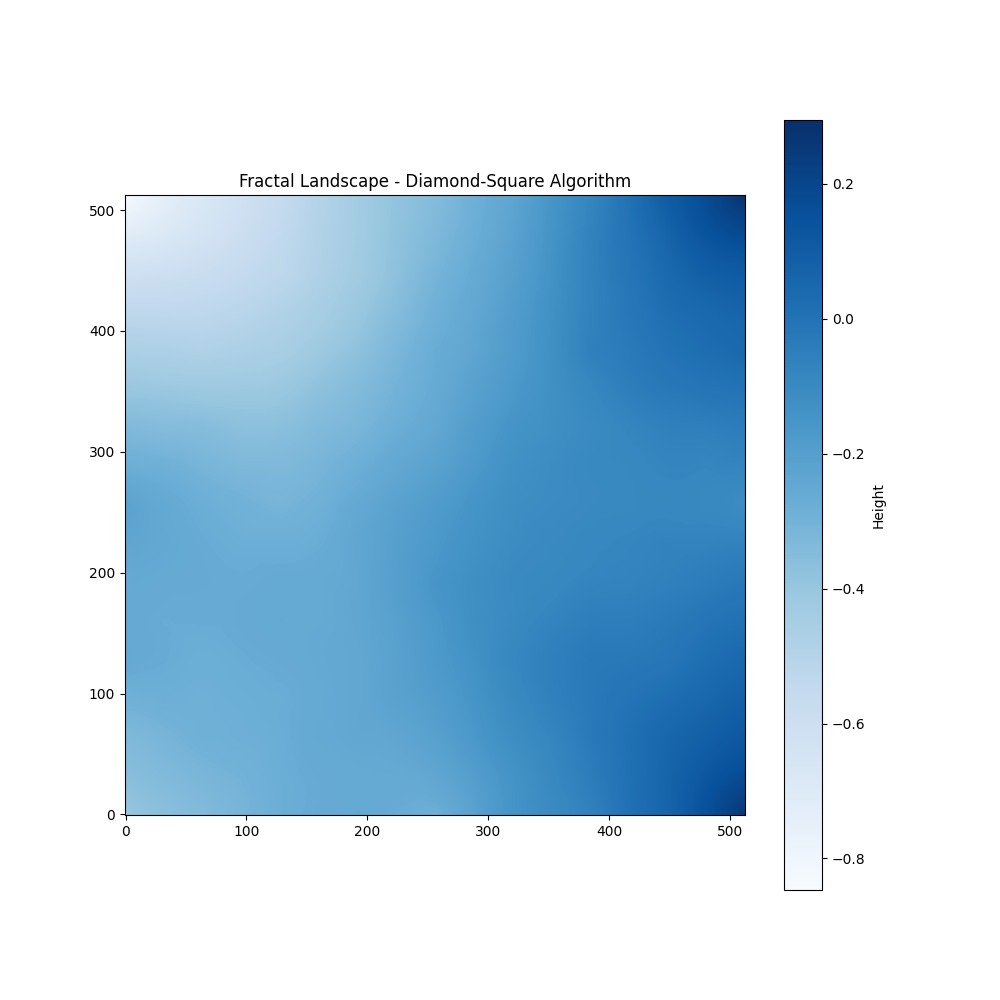
\includegraphics[width=0.7\linewidth]{Blues_9_0.3.png}
    \caption{Roughness = 0.3}
\end{figure}

\begin{figure}[H]
    \centering
    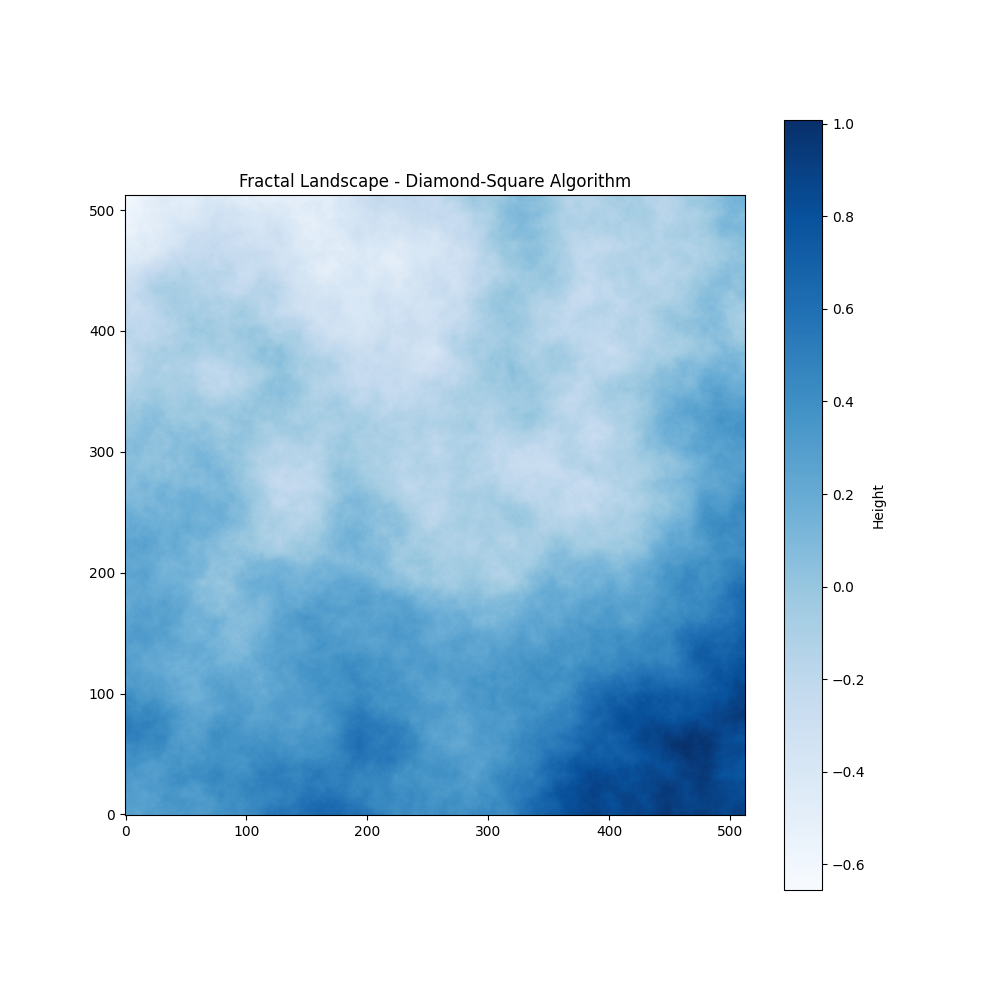
\includegraphics[width=0.7\linewidth]{Blues_9_0.6.png}
    \caption{Roughness = 0.6}
\end{figure}

\begin{figure}[H]
    \centering
    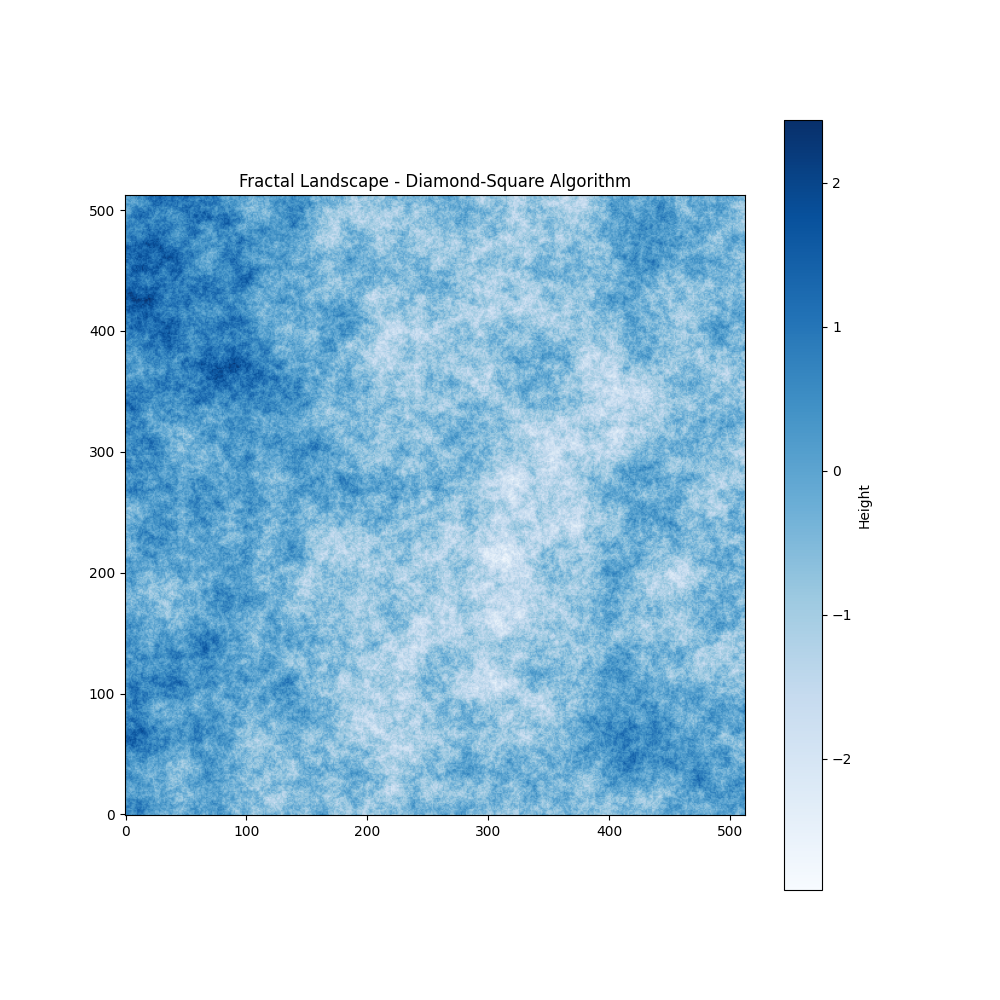
\includegraphics[width=0.7\linewidth]{Blues_9_0.9.png}
    \caption{Roughness = 0.9}
\end{figure}

\vspace{1cm}

\section{Przykłady zastosowań interpolacji fraktalnej}

\begin{itemize}
    \item \textbf{Generowanie krajobrazów}: Interpolacja fraktalna jest szeroko stosowana w symulacji realistycznych terenów, takich jak góry, doliny, wyspy czy oceany.
    \item \textbf{Grafika komputerowa}: Wykorzystywana w grach, filmach i wizualizacjach do generowania powierzchni nieregularnych.
    \item \textbf{Analiza sygnałów}: Przydatna do analizy danych, które mają charakter fraktalny (np. sejsmologia, turbulencje w atmosferze).
    \item \textbf{Modelowanie procesów naturalnych}: Modelowanie linii brzegowych, wzrostu roślin czy przepływów rzecznych.
\end{itemize}

\vspace{1cm}

\section{Podsumowanie}

Generowanie krajobrazów za pomocą interpolacji fraktalnej, w tym algorytmu Diamond-Square, umożliwia tworzenie złożonych i realistycznych struktur o nieregularnej geometrii. Analiza tych krajobrazów przy użyciu wymiarów Minkowskiego i Hausdorffa pozwala na głębsze zrozumienie ich właściwości matematycznych. Dzięki prostocie implementacji i szerokim możliwościom zastosowania, metoda ta znajduje zastosowanie w wielu dziedzinach, od grafiki komputerowej po nauki przyrodnicze i inżynierię.


\end{document}
